%!Mode:: "TeX:UTF-8"
\documentclass[a4paper,11pt,UTF8]{ctexart}

\usepackage{indentfirst} %缩进
\usepackage{xeCJK}    %使用系统字体
\usepackage{fancyhdr} %自定义页眉页脚
\pagestyle{empty}                   %不设置页眉页脚
\usepackage{amsmath, amsthm, amssymb, amsfonts} %数学公式
\usepackage[a4paper,left=3cm,right=3cm,top=3cm,bottom=3cm]{geometry}
%\usepackage[tmargin=1in,bmargin=1in,lmargin=1.25in,rmargin=1.25in]{geometry}.
\usepackage{booktabs} %插入表格
\usepackage[section]{placeins} %避免浮动
\usepackage{listings} %插入代码
\usepackage{ctex}     %中文宏包
\usepackage[svgnames, table]{xcolor} %彩色表格
\usepackage{algorithm}          %伪代码
\usepackage{algorithmicx}
\usepackage{algpseudocode}
\usepackage{algorithm,algpseudocode,float}
\usepackage{lipsum}
\usepackage{enumitem}           %调整列举环境
\usepackage{url}
\usepackage{fontspec,xunicode}
\defaultfontfeatures{Mapping=tex-text} %如果没有它,会有一些 tex 特殊字符无法正常使用,比如连字符。

\usepackage{graphicx}
\graphicspath{{imgs/}}
\usepackage{verbatim}
%%%%%%%%%%%%%%%%%%%%%%%%%%%%%%%%%%%%%%%%%%%%%%%%%%%%%%%%%%%%%%%%
% 缩进及行间距
%%%%%%%%%%%%%%%%%%%%%%%%%%%%%%%%%%%%%%%%%%%%%%%%%%%%%%%%%%%%%%%%
\setlength{\parindent}{22pt} %重新定义缩进长度
\setlength{\baselineskip}{20pt}  %定义行间距
%\renewcommand{\baselinestretch}{1.1} %定义行间距

%%%%%%%%%%%%%%%%%%%%%%%%%%%%%%%%%%%%%%%%%%%%%%%%%%%%%%%%%%%%%%%%
% 列表设置
%%%%%%%%%%%%%%%%%%%%%%%%%%%%%%%%%%%%%%%%%%%%%%%%%%%%%%%%%%%%%%%%
\setenumerate{fullwidth,itemindent=\parindent,listparindent=\parindent,itemsep=0ex,partopsep=0pt,parsep=0ex}
\setenumerate[2]{label=\alph*),leftmargin=1.5em}  %二级item设置
\setitemize{itemindent=38pt,leftmargin=0pt,itemsep=-0.4ex,listparindent=26pt,partopsep=0pt,parsep=0.5ex,topsep=-0.25ex}
\setdescription{itemindent=38pt,leftmargin=0pt,itemsep=-0.4ex,listparindent=26pt,partopsep=0pt,parsep=0.5ex,topsep=-0.25ex}

%%%%%%%%%%%%%%%%%%%%%%%%%%%%%%%%%%%%%%%%%%%%%%%%%%%%%%%%%%%%%%%%
% 图的标题行间距设置
%%%%%%%%%%%%%%%%%%%%%%%%%%%%%%%%%%%%%%%%%%%%%%%%%%%%%%%%%%%%%%%%
\newcommand{\bottomcaption}{%
\setlength{\abovecaptionskip}{6pt}%
\setlength{\belowcaptionskip}{6pt}%
\caption}


%%%%%%%%%%%%%%%%%%%%%%%%%%%%%%%%%%%%%%%%%%%%%%%%%%%%%%%%%%%%%%%%
% 字体定义
%%%%%%%%%%%%%%%%%%%%%%%%%%%%%%%%%%%%%%%%%%%%%%%%%%%%%%%%%%%%%%%%
\setmainfont{Times New Roman}  %默认英文字体.serif是有衬线字体sans serif无衬线字体
\setmonofont{Consolas}
\setCJKmainfont[ItalicFont={楷体}, BoldFont={黑体}]{宋体}%衬线字体 缺省中文字体为
\setCJKsansfont{黑体}
\punctstyle{hangmobanjiao}
%-----------------------xeCJK下设置中文字体------------------------------%
\setCJKfamilyfont{song}{SimSun}                             %宋体 song
\newcommand{\song}{\CJKfamily{song}}
\setCJKfamilyfont{fs}{FangSong}                      %仿宋  fs
\newcommand{\fs}{\CJKfamily{fs}}
\setCJKfamilyfont{ktgb}{KaiTi}                      %楷体2312 ktgb
\newcommand{\ktgb}{\CJKfamily{ktgb}}
\setCJKfamilyfont{yh}{Microsoft YaHei}                    %微软雅黑 yh
\newcommand{\yh}{\CJKfamily{yh}}
\setCJKfamilyfont{hei}{SimHei}                              %黑体  hei
\newcommand{\hei}{\CJKfamily{hei}}
\setCJKfamilyfont{hwxk}{STXingkai}                                %华文行楷  hwxk
\newcommand{\hwxk}{\CJKfamily{hwxk}}
%------------------------------设置字体大小------------------------%
\newcommand{\shiyanbaogao}{\fontsize{36pt}{\baselineskip}\selectfont}
\newcommand{\chuhao}{\fontsize{42pt}{\baselineskip}\selectfont}     %初号
\newcommand{\xiaochuhao}{\fontsize{36pt}{\baselineskip}\selectfont} %小初号
\newcommand{\yihao}{\fontsize{28pt}{\baselineskip}\selectfont}      %一号
\newcommand{\erhao}{\fontsize{21pt}{\baselineskip}\selectfont}      %二号
\newcommand{\xiaoerhao}{\fontsize{18pt}{\baselineskip}\selectfont}  %小二号
\newcommand{\sanhao}{\fontsize{15.75pt}{\baselineskip}\selectfont}  %三号
\newcommand{\sihao}{\fontsize{14pt}{\baselineskip}\selectfont}       %四号
\newcommand{\xiaosihao}{\fontsize{12pt}{\baselineskip}\selectfont}  %小四号
\newcommand{\wuhao}{\fontsize{10.5pt}{\baselineskip}\selectfont}    %五号
\newcommand{\xiaowuhao}{\fontsize{9pt}{\baselineskip}\selectfont}   %小五号
\newcommand{\liuhao}{\fontsize{7.875pt}{\baselineskip}\selectfont}  %六号
\newcommand{\qihao}{\fontsize{5.25pt}{\baselineskip}\selectfont}    %七号

%%%%%%%%%%%%%%%%%%%%%%%%%%%%%%%%%%%%%%%%%%%%%%%%%%%%%%%%%%%%%%%%
% 图题字体大小相同
%%%%%%%%%%%%%%%%%%%%%%%%%%%%%%%%%%%%%%%%%%%%%%%%%%%%%%%%%%%%%%%%
\usepackage{caption}
\captionsetup{font={footnotesize}}   % footnotesize = 9pt
\captionsetup[lstlisting]{font={footnotesize}}

%%%%%%%%%%%%%%%%%%%%%%%%%%%%%%%%%%%%%%%%%%%%%%%%%%%%%%%%%%%%%%%%
% 重定义枚举编号为 1),2)...
%%%%%%%%%%%%%%%%%%%%%%%%%%%%%%%%%%%%%%%%%%%%%%%%%%%%%%%%%%%%%%%%
\renewcommand{\labelenumi}{\theenumi)}


%%%%%%%%%%%%%%%%%%%%%%%%%%%%%%%%%%%%%%%%%%%%%%%%%%%%%%%%%%%%%%%%
% 重定义section标题
%%%%%%%%%%%%%%%%%%%%%%%%%%%%%%%%%%%%%%%%%%%%%%%%%%%%%%%%%%%%%%%%
\CTEXsetup[format={\sihao\CJKfamily{zhhei}\zihao{4}},number={\chinese{section}},name={,、~},aftername={},indent={0pt},beforeskip={6pt},afterskip={6pt},format+={\flushleft}]{section}
\CTEXsetup[format={\Large\bfseries\CJKfamily{zhkai}\zihao{5}},name={(,)},number={\chinese{subsection}},aftername={},indent={22pt},beforeskip={14pt},afterskip={2pt}]{subsection}
\CTEXsetup[number={\chinese{section}},name={附录, ~~ }]{appendix}



%%%%%%%%%%%%%%%%%%%%%%%%%%%%%%%%%%%%%%%%%%%%%%%%%%%%%%%%%%%%%%%%
% 标题名称中文化
%%%%%%%%%%%%%%%%%%%%%%%%%%%%%%%%%%%%%%%%%%%%%%%%%%%%%%%%%%%%%%%%
\renewcommand\figurename{\hei 图}
\renewcommand\tablename{\hei 表}
\renewcommand\lstlistingname{\hei 代码}
\renewcommand{\algorithmicrequire}{\textbf{输入:}}
\renewcommand{\algorithmicensure}{\textbf{输出:}}
\newtheorem{define}{定义}

%%%%%%%%%%%%%%%%%%%%%%%%%%%%%%%%%%%%%%%%%%%%%%%%%%%%%%%%%%%%%%%%
% 代码设置
%%%%%%%%%%%%%%%%%%%%%%%%%%%%%%%%%%%%%%%%%%%%%%%%%%%%%%%%%%%%%%%%
\lstset{
 columns=fixed,
 numbers=left,                                        % 在左侧显示行号
 numberstyle=\tiny\color{gray},                       % 设定行号格式
 frame=single,                                        % 单线背景边框
 breaklines=true,                                     % 设定LaTeX对过长的代码行进行自动换行
 keywordstyle=\color[RGB]{40,40,255},                 % 设定关键字颜色
 numberstyle=\footnotesize\color{darkgray},
 commentstyle=\it\color[RGB]{0,96,96},                % 设置代码注释的格式
 stringstyle=\rmfamily\slshape\color[RGB]{128,0,0},   % 设置字符串格式
 showstringspaces=false,                              % 不显示字符串中的空格
 language=java,                                        % 设置语言
 basicstyle=\linespread{1.0}\xiaowuhao\ttfamily,                      % 字体字号
 %lineskip=10pt,
 %baselinestretch=1,
}

%%%%%%%%%%%%%%%%%%%%%%%%%%%%%%%%%%%%%%%%%%%%%%%%%%%%%%%%%%%%%%%%
% 伪代码分页
%%%%%%%%%%%%%%%%%%%%%%%%%%%%%%%%%%%%%%%%%%%%%%%%%%%%%%%%%%%%%%%%
\makeatletter
\renewcommand{\ALG@name}{算法}
\newenvironment{breakablealgorithm}
  {% \begin{breakablealgorithm}
   \begin{center}
     \refstepcounter{algorithm}% New algorithm
     \hrule height.8pt depth0pt \kern2pt% \@fs@pre for \@fs@ruled
     \renewcommand{\caption}[2][\relax]{% Make a new \caption
       {\raggedright\textbf{\ALG@name~\thealgorithm} ##2\par}%
       \ifx\relax##1\relax % #1 is \relax
         \addcontentsline{loa}{algorithm}{\protect\numberline{\thealgorithm}##2}%
       \else % #1 is not \relax
         \addcontentsline{loa}{algorithm}{\protect\numberline{\thealgorithm}##1}%
       \fi
       \kern2pt\hrule\kern2pt
     }
  }{% \end{breakablealgorithm}
     \kern2pt\hrule\relax% \@fs@post for \@fs@ruled
   \end{center}
  }
\makeatother

\begin{document}
\xiaosihao\song

\begin{titlepage}
\center{\yihao{\hwxk{中国科学技术大学微电子学院}}}
\vspace{1cm}
\begin{comment}
\begin{figure}[H]
	\centering
	%bmeps test.jpg test.eps
	\includegraphics[scale=0.4]{1.eps}
	\caption{图片标题}
	\label{figl}
\end{figure}
\end{comment}
\begin{figure}[!htbp]
	\centering
	
\includegraphics[scale=0.5]{logo.png}
\end{figure}
%\vspace{6cm}
\center{\shiyanbaogao{\ktgb{实~验~报~告}}}
\vspace{3cm}

\begin{center}
\begin{large}
\begin{tabular}{rc}
\xiaoerhao{\hei{学\qquad 号}}& \hspace{1.7cm}\xiaoerhao{\hei{PB17061124\hspace{1.7cm}}} \\
\cline{2-2}\\
\xiaoerhao{\hei{姓\qquad 名}}& \xiaoerhao{\hei{胡~睿}}\\
\cline{2-2}\\
\xiaoerhao{\hei{专\qquad 业}}& \xiaoerhao{\hei{电子科学技术系}}\\
\cline{2-2}\\
\xiaoerhao{\hei{课程名称}}& \xiaoerhao{\hei{微~机~原~理~与~嵌~入~式~系~统}}\\
\cline{2-2}\\
\xiaoerhao{\hei{指导教师}}& \xiaoerhao{\hei{何~力}}\\
\cline{2-2}\\
\end{tabular}
\end{large}
\end{center}
\vfill \hfill
\end{titlepage}
\clearpage

\centerline{\\[10pt]\erhao{\fs{中~国~科~学~技~术~大~学}}}
\centerline{\\[10pt]\yihao{\fs{实  ~~ 验  ~~ 报  ~~ 告}}}

\leftline{\\[10pt]\sihao{\hei{\hspace{1.5em} 学生姓名:胡睿 \hfill 学号:PB17061124 \hfill 指导教师:何力 }}}

\setlength{\parskip}{6pt}  %定义段间距

\section{实验名称: 基本谱减法语音信号降噪的设计与实现 }
\section{实验目的:}

1.学习使用Matlab进行语音信号处理;\par 
2.学习谱减法的基本思想;\par 
3.学习对语音信号加窗、分帧及FFT、IFFT;\par 
4.使用谱减法实现对语音信号的增强. 

\section{实验原理:}

设语音信号为$x(n)$,加窗分帧处理后第i帧信号为$x_i(n)$,帧长为N。语音帧$x_i(n)$的DFT为$X_i(k)$,其幅度为$|X_i(k)|$,相角为$\angle X_i(k)$,$\angle X_i(k)=arctan[\frac{Im(X_i(k))}{Re(X_i(k))}]$。\par 

一般,可以假设语音信号最前面一段是噪声段,并可以从中获取噪声的平均能量,记为$E_N(k)$。设噪声段的帧数为$N_n$,则$E_N(k)$的计算可以采用:$E_N(k)=\frac{1}{N_n}\sum_{i=1}^{N_n}|X_i(k)|^2$。\par 

谱减法的基本思想是按帧计算:
	\begin{equation}
	|X_i(k)|^2 = \left \{
	\begin{array}{rl}
		|X_i(k)|^2-a\cdot E_N(k) & |X_i(k)|^2\geq a\cdot E_N(k) \\
		b\cdot |X_i(k)|^2        & |X_i(k)|^2\textless a\cdot E_N(k)
	\end{array}
	\right. 
	\nonumber
	\end{equation}
	
式中a和b是两个常数,分别称之为过减因子和增益补偿因子;然后利用语音信号对相位的不灵敏特性,把谱减后的幅值$X_i(k)$结合先前计算并保存的相角$\angle X_i(k)$再经过FFT反变换,即IFFT,可以得到谱减后的语音序列$x_i(n)$。\par 

基本谱减法降噪的基本原理如下图所示:
\begin{figure}[!htbp]
	\centering
	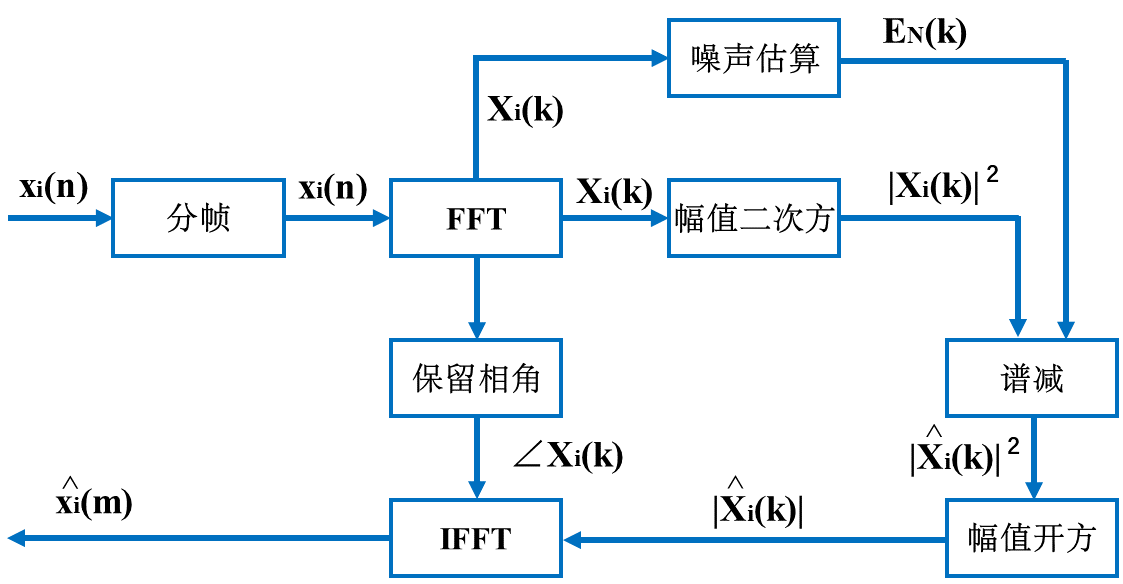
\includegraphics[width=\textwidth]{principle}
	\bottomcaption{\xiaowuhao{基本谱减法原理图}}
\end{figure}

\section{实验内容:}

根据上述基本谱减法的思想,设计程序实现含噪语音信号的增强。含噪语音信号可以采用干净语音信号加噪声(例如:高斯白噪声)的做法得到,加噪声时控制一定的信噪比。

\section{实验器材(设备、元器件):}

Matlab、visual studio

\section{实验步骤:}

一、编程计算恰当的a、b取值\par 
(1)当原信号和增强后的信号均方差最小的时候增强效果最好,因此在不同的a、b取值下分别对原信号和增强后的信号求均方差并绘制三维图像;\par 
(2)求出图像的最低点坐标;\par 
(3)得到a、b的最恰当取值。\par 

二、利用第一步计算得到的a、b取值对信号进行谱减法降噪。


\section{实验结果与分析(含重要数据结果分析或核心代码流程分析):}
一、计算恰当的a、b取值:
\begin{itemize}
	\item 计算残差文件 :residual.m
	\item 处理信号文件 :bluesky1.wav
\end{itemize}

\begin{lstlisting}[caption={计算恰当的a、b取值},captionpos=b]
clear all;
close all;

%sound(enhanced,fs);pause(5);

\end{lstlisting}

运行结果:\par
\begin{figure}[!htbp]
	\centering
	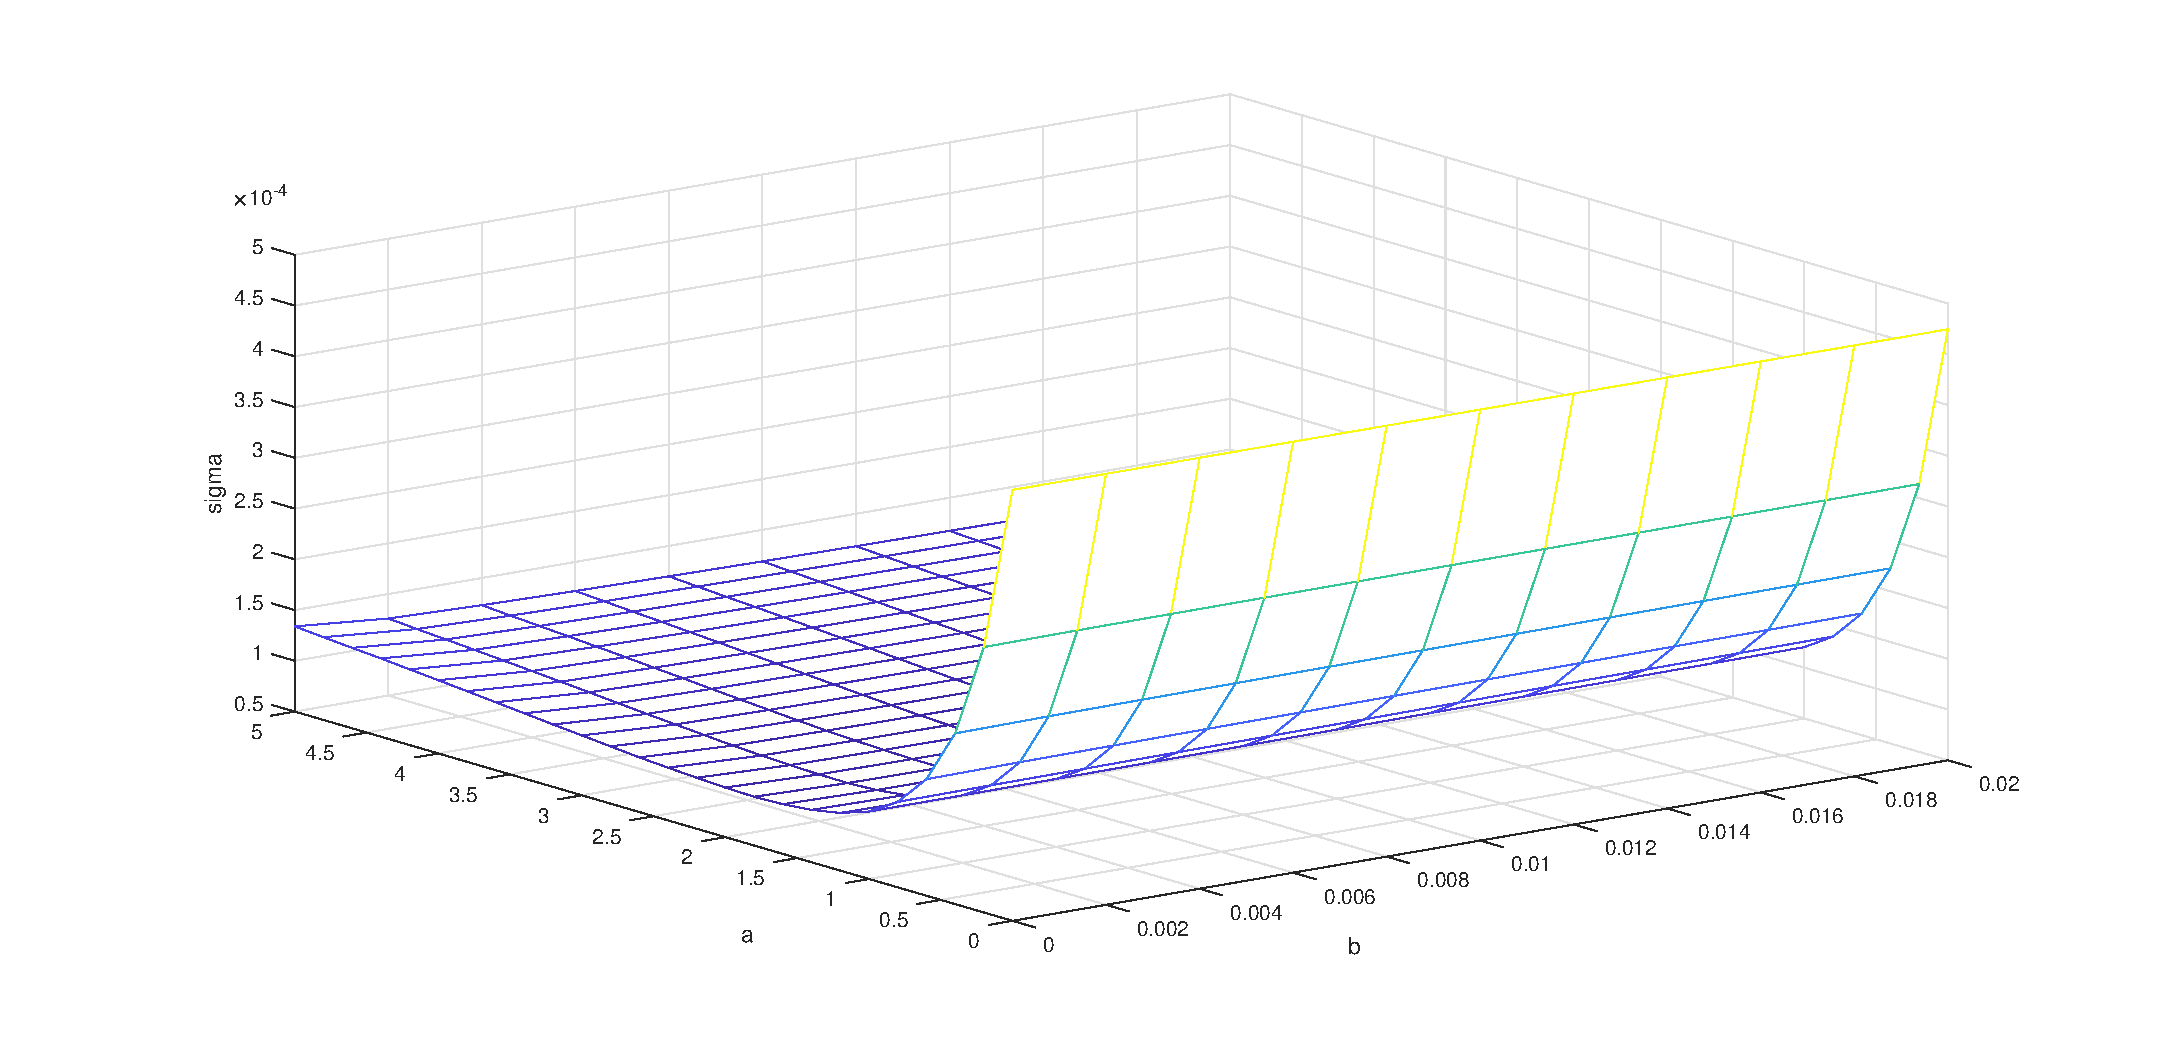
\includegraphics[width=\textwidth]{residual.eps}
	\bottomcaption{\xiaowuhao{不同a、b下的均方差}}
\end{figure}

运行结果图2分析:\par
1.得到了不同a、b下的均方差的三维图像;\par
2.为了使得图像更加直观,我们可以使用view([0,0])命令得到图像的正视图,正视图可以直观地看到b的取值对均方差的影响,我们可以使用view([-90,0])命令得到图像的左视图,左视图可以直观地看到a的取值对均方差的影响。



\section{总结及心得体会:}

1.学习使用Matlab进行语音信号处理,熟悉了audioread、fft等数字信号处理常用函数的使用,提升了发现问题分析问题解决问题的能力,练习使用matlab生成一定信噪比的噪声并添加进入语音信号当中;\par 
2.学习了谱减法的基本思想;\par 
3.学习对语音信号加窗、分帧及FFT、IFFT;\par 
4.分析了恰当的a、b取值并使用谱减法实现对语音信号的降噪使得降噪效果良好、语音波形失真较小。

\begin{comment}
\section{对本实验过程及方法、手段的改进建议:}

(自行填写。必须写点什么,不能写“无”)

(注意:八,九部分能反映出实验的态度、方法和效果,应重点阐述,字数勿少,独立完成,勿参考其他报告,避免雷同)

\begin{appendix}

\section{表格示例}
\begin{table}[!h!tbp]
\caption{一个简单的表格}\label{tab1}
  \centering
  \begin{tabular}{|l|c|c|}
	\hline
	功能          &WEB         &APP         \\ \hline
	注册          &$\surd$     &$\surd$     \\ \hline
	登录          &$\surd$     &$\surd$     \\ \hline
	推送          &$\times$    &$\surd$     \\ \hline
\end{tabular}
\end{table}

\begin{table}[!h!tbp]
\caption{自定义表格}\label{tab2}
  \centering
\begin{tabular*}{0.75\textwidth}{@{\extracolsep{\fill}}lcc}
    \toprule
    功能          &WEB         &APP         \\
    \midrule
    注册          &$\surd$     &$\surd$     \\
    登录          &$\surd$     &$\surd$     \\
    推送          &$\times$    &$\surd$     \\
    \bottomrule
\end{tabular*}
\end{table}

\section{伪代码示例}

\begin{algorithm}
\caption{某个算法}
\begin{algorithmic}[1]  %每行显示行号
\Require 某个输入
\Ensure 某个输出
\Function {函数名} {参数列表}
    \State 某个变量  $\gets$ 某个变量
\EndFunction
\end{algorithmic}
\end{algorithm}

\section{字体示例}
\hei{黑体}
\hwxk{华文行楷}

\end{appendix}
\end{comment}
\end{document}
